\artikel{Archiv: Griechische Buchstaben}
{Wir gehen in die sechste Folge fächerübergreifend beliebten Sammelserie der griechischen Buchstaben.
	Schnell ausscheiden und ins Sammelalbum einkleben oder mit Freunden tauschen!}
{\vspace*{-1.5\baselineskip}\begin{center}
		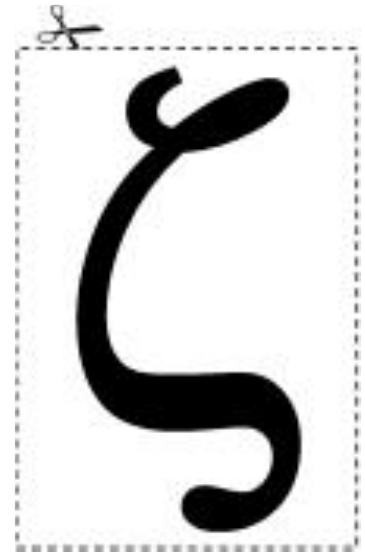
\includegraphics[scale=0.4]{grafik/zeta.png}
	\end{center}
	\flushleft
	Wir verlassen die seichten Gebilde der Anfängerbuchstaben und
	nähern uns den etwas unbekannteren Buchstaben, die nicht so
	häufig verwendet werden. Aber trotzdem sollte in der vollständigen
	Sammlung der Griechischen Buchstaben das $\zeta$ nicht fehlen,
	schon alleine, um etwas humanistische Bildung zu demonstrieren.

	\subsection*{Verwendung}

	Es gab mal einen berühmten Mathematiker namens Riemann, der hat eine Funktion
	erfunden und diese $\zeta$-Funktion genannt. Sie stellt die Verteilung
	der Primzahlen als Formel dar. Und es gab auch mal ein paar Informatiker, die
	haben ein Betriebssystem mit diesem Namen versehen, das früher auch mals BeOS
	bekannt war.
	Der Autobauer Lancia hat ein Auto namens $\zeta$ herausgebracht.
	Viel mehr Beispiele der Verwendung gibt es eigentlich nicht, da dieser
	Buchstabe so unbekannt ist, verwenden ihn nur wenige.

	\subsection*{Zubereitung}
	Man nehme einen Stift, zum Beispiel den Lieblingsfüller
	mit gefederter und ergonomisch geformter Grundmulde.
	Mit diesem nun das Papier berühren und dabei die Bewegungen
	ausführen, die zum Erscheinen des $\zeta$ auf selbigen
	führen. Diese wären: eine kleine Schleife gegen den Uhrzeigersinn,
	dann eine große hintenangehängt. Wenn eine halbe
	Umdrehung vollbracht ist, die Richtung ändern und einen kleinen Schlenker
	unten anhängen. Fertig ist das $\zeta$ und kann fortan bewundert werden.

	\subsection*{Empfehlung}
	Da der geübte Laie bei der Zubereitung des $\zeta$ leicht eine
	Sehnenscheidenentzündung bekommen kann, empfehlen wir, eine ausgewogene
	Mischung aus $\zeta$ und anderen Buchstaben zu verwenden. Sieht dann auch nicht so
	eintönig aus.}
{Arne Pottharst}\vfill
\small Dieser Artikel erschien ursprünglich im Juni 2006 und steht daher nicht unter
CC-BY-SA.
